\chapter{General Information}

\section{Clearing Error Messages}

Errors are displayed on \textbf{line 1} of the screen, indicated by the word \textbf{ERROR} followed by an error code.

The error codes are grouped in a separate \textbf{error list}, which is located in the machine's electrical cabinet.

\subsection{Important Note}

The root cause of an error must always be resolved before continuing work on the machine and its control system.

\subsection{Clearing Control and Programming Errors}

\begin{itemize}
    \iconitem{Control and programming errors (e.g., incorrect operations) can be cleared using the \textbf{CLEAR} button.}{clear.jpg} 
\end{itemize}

\subsection{Clearing Hardware and Interface Errors}

Hardware and interface errors can be cleared by pressing the following three buttons in sequence:

\begin{itemize}
    \iconitem {\textbf{MANUAL}}{manual.jpg}
    \vspace{.6cm}
    \iconitem{ \textbf{CLEAR CONTR.}}{clear_contr.jpg}
    \vspace{.6cm}
    \iconitem {\textbf{CLEAR}}{clear.jpg}
\end{itemize}

\vspace{.5cm}

\noindent (It is not necessary to press the \textbf{MANUAL} button when the system is already operating in manual mode.)

Pressing both \textbf{MANUAL} and \textbf{CLEAR CONTR.} simultaneously while a program is running will cause the program to stop. The program must be restarted once the root cause of the error has been resolved (see \textbf{Section 7.1.1}).

\newpage
\section{Step-by-Step Mode (MANUAL)}

\begin{itemize}
    \iconitem {Press the \textbf{MANUAL} button.}{manual.jpg}
\end{itemize}

The following display appears on the screen:

\begin{figure}[h]
    \centering
    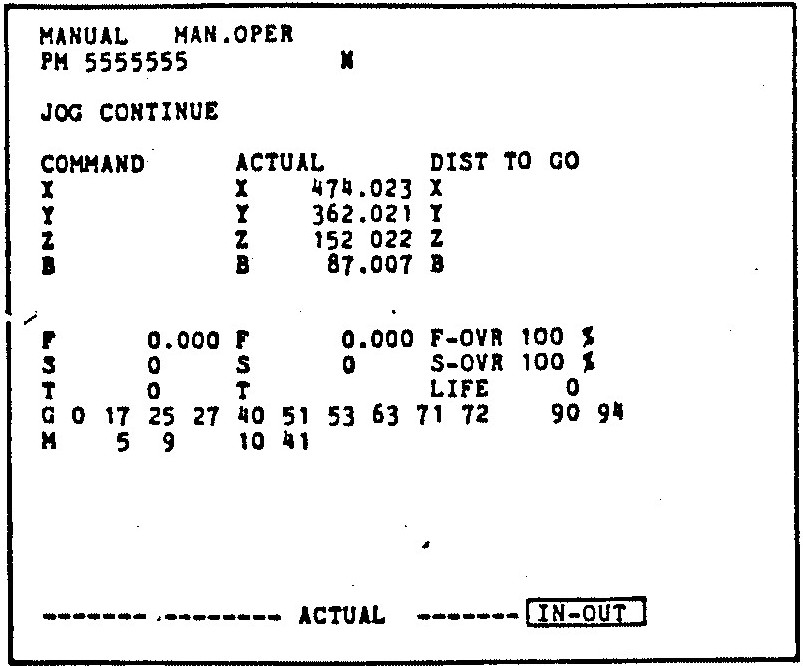
\includegraphics[width=0.7\textwidth]{manual_screen.jpg}
    \caption{Display in Manual Mode}
\end{figure}

\subsection{Movement at a Low Feed Rate}

A fixed feed rate is stored in memory for step-by-step mode as part of the machine constants. This value can be modified within the range of **0-100\%** using the feed rate correction buttons.

\procedure

\marginnoteicon[.8cm]{18.7cm}{feed_correction.jpg}[-.5cm]

\begin{itemize}
    \item Press the feed rate correction buttons.
\end{itemize}

\begin{itemize}
    \item Press the button for the corresponding axis.
\end{itemize}

The machine axis moves at the set feed rate as long as the button for that axis remains pressed.

During movement, \textbf{JOG +} or \textbf{JOG -} is displayed under \textbf{COMMAND}.

The feed rate percentage value is displayed on \textbf{line 13} of the screen.

\subsubsection*{Simultaneous Movement of Two Axes}

It is also possible to move two machine axes simultaneously.

\marginnoteicon[4.5cm]{20cm}{axis_movement.jpg}[-2.7cm]

\begin{itemize}
    \item An axis cannot move if both \textbf{"+"} and \textbf{"-"} buttons of the same axis are pressed at the same time.
    \item An axis will not move if more than two axes are activated simultaneously.
\end{itemize}

\newpage
\subsection{Adjustable Incremental Movement (Incremental Mode)}

For incremental movement, the incremental step value can be selected using the incremental movement buttons.

Depending on the selected button (1, 10, 100, or 1000), the movement will be executed in **1, 10, 100, or 1000 increments**.

\begin{center}
    1 increment = 0.001 mm or 0.0001 inch.
\end{center}

\procedure

\begin{itemize}
    \item Press one of the **increment selection buttons**: 1, 10, 100, or 1000.
\end{itemize}

\marginnoteicon[.8cm]{7.6cm}{incremental_buttons.jpg}[-.5cm]

\noindent The selected incremental movement value is displayed on **line 4** of the screen.

\begin{itemize}
    \item Press the button for the corresponding axis.
\end{itemize}

The machine axis moves by the selected increment.

Once the incremental movement has been executed, **0** appears on the screen below \textbf{DIST TO GO}.

\marginnoteicon[4cm]{9cm}{axis_movement.jpg}[-2cm]

An axis will not move if:
\begin{itemize}
    \item More than one axis button is pressed simultaneously.
    \item Both "+" and "-" buttons for the same axis are pressed at the same time.
\end{itemize}

\subsubsection*{Returning to Continuous Feed}

Once the incremental feed procedure is complete:

\begin{itemize}
    \iconitem {Press the button shown to the right to initialize continuous feed in step-by-step mode.}{continuous_feed.jpg}
\end{itemize}

\newpage

\subsection{Manual Control Panel (REMOTE PANEL)}

Selection of the manual control panel.

\procedure

\begin{itemize}
    \iconitem {Press the \textbf{MANUAL} button.}{manual.jpg}
\end{itemize}

\vspace{.5cm}
\begin{itemize}
    \iconitem {Press the \textbf{MENU} button.}{menu.jpg}
\end{itemize}
\vspace{.5cm}
The main command submenu appears on the screen:

\begin{figure}[h]
    \centering
    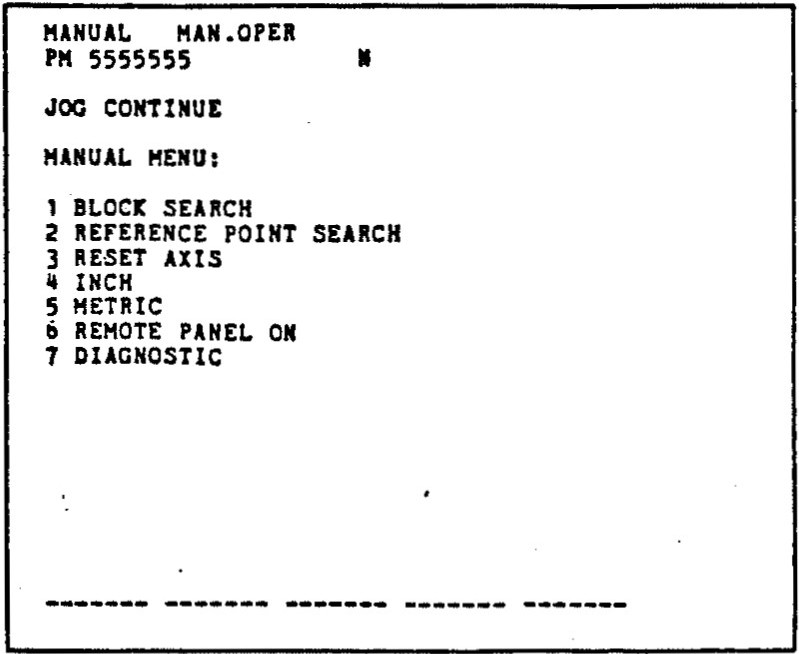
\includegraphics[width=0.6\textwidth]{manual_menu.jpg}
    \caption{Main Command Menu}
\end{figure}

\begin{itemize}
    \item Press key \textbf{6} on the numeric keypad to select \textbf{REMOTE PANEL ON}.
\end{itemize}

The following display appears on the screen:

\begin{figure}[h]
    \centering
    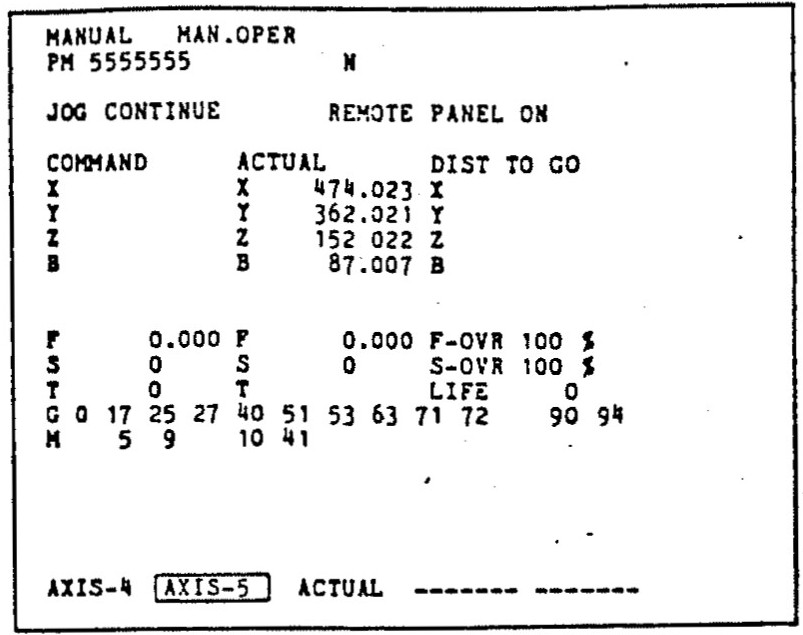
\includegraphics[width=0.6\textwidth]{remote_panel_display.jpg}
    \caption{Display with Remote Panel Activated}
\end{figure}

\newpage
\notes

After selecting the manual control panel, the active button is indicated by a \textbf{red LED}. The buttons and their functions are identical to those on the main control panel.

However, instead of feed rate correction buttons, the manual control panel is equipped with a \textbf{potentiometer}.

To use the manual control panel after selection, it is always necessary to press and hold one of the \textbf{safety buttons} located on the side of the panel.

The \textbf{EMERGENCY STOP} switch remains active at all times.

\marginnoteicon[2.5cm]{3cm}{potentiometer.jpg}[-2cm]

\subsection{Metric and Inch Measurement Systems (METRIC/INCH)}

Dimensions and feed rates can be entered in either \textbf{metric} or \textbf{inches}.

The measurement system selected at the beginning of a program must remain in use until the end of the program for each machining operation.

The measurement system used by the control, and stored in the \textbf{machine constants memory}, is always displayed on the screen \textbf{after machine startup}.

If the program requires a change in the measurement system, the operator must also enter the \textbf{tool data} in the \textbf{new unit system} after switching.

\textbf{Previously stored programs cannot be executed} after changing the unit system, as no automatic conversion is performed in memory. They can only be executed again after switching back to the original unit system used when they were programmed.

However, it is possible to \textbf{call stored programs} before changing the unit system and save them again after the change. In this case, dimensions and feed rates are automatically converted to the new system, allowing the execution of existing programs in the new unit system.

\textbf{It is essential to re-reference the machine axes} after every unit system change (see \textbf{Section 1.2}).

\procedure

\begin{itemize}
    \iconitem {Press the \textbf{MANUAL} button.}{manual.jpg}
\end{itemize}

\vspace{.5cm}

\begin{itemize}
    \iconitem {Press the \textbf{MENU} button.}{menu.jpg}
\end{itemize}

\newpage

The main command submenu appears on the screen:

\begin{figure}[h]
    \centering
    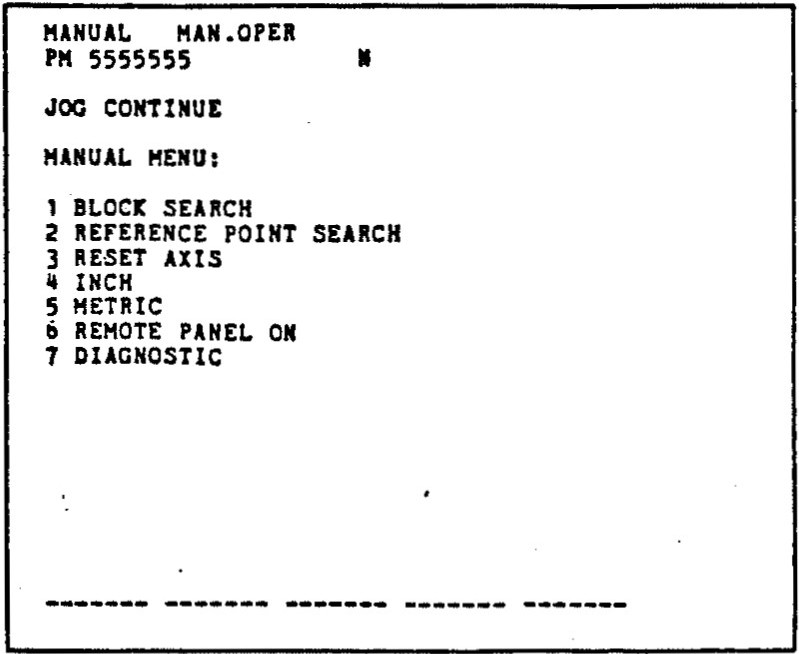
\includegraphics[width=0.7\textwidth]{manual_menu.jpg}
    \caption{Main Command Menu}
\end{figure}

\begin{itemize}
    \item Press key \textbf{4} on the numeric keypad to select \textbf{INCH} or key \textbf{5} to select \textbf{METRIC}.
\end{itemize}

\begin{itemize}
    \item The display will then show \textbf{G70 (INCH)} or \textbf{G71 (METRIC)} on the line for G functions.
\end{itemize}

\notes

For practical reasons, it is possible that the other unit system is more commonly used. In this case, the \textbf{machine constants stored in memory} must be modified accordingly so that the preferred unit system is automatically activated when the machine and control system are started.

\newpage

\subsection{Reference Point Search During Machine Operation (REFERENCE POINT SEARCH)}

It may be necessary to search for the reference point on one or more machine axes during operation (e.g., for verification purposes).

The reference points of the different machine axes are generally set to determine a new workpiece origin (see \textbf{Section 3.4.1}).

\procedure

\begin{itemize}
    \iconitem {Press the \textbf{MANUAL} button.}{manual.jpg}
\end{itemize}

\vspace{.5cm}

\begin{itemize}
    \iconitem {Press the \textbf{MENU} button.}{menu.jpg}
\end{itemize}
\vspace{.5cm}
The main command submenu appears on the screen:

\begin{figure}[h]
    \centering
    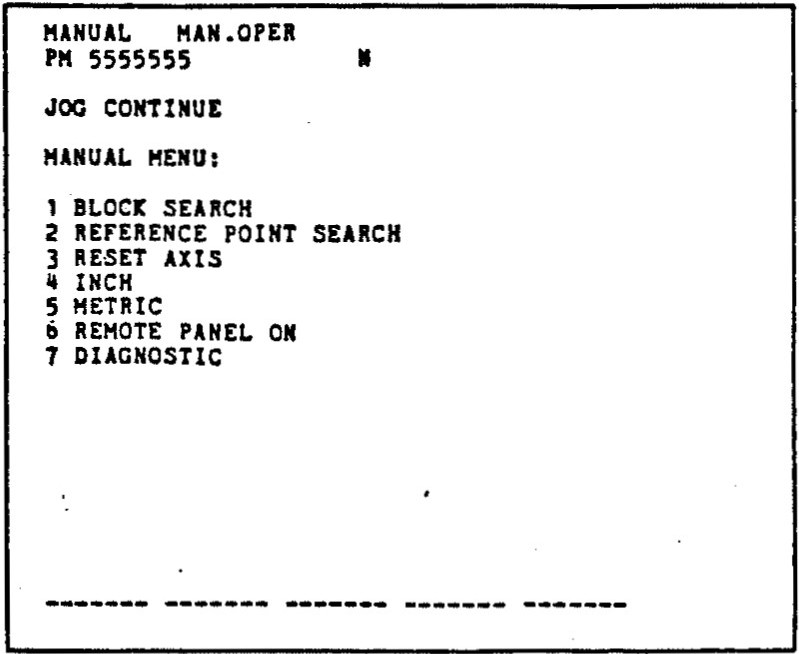
\includegraphics[width=0.6\textwidth]{manual_menu.jpg}
    \caption{Main Command Menu}
\end{figure}

\begin{itemize}
    \item Press key \textbf{2} on the numeric keypad to select \textbf{REFERENCE POINT SEARCH}.
\end{itemize}

\begin{itemize}
    \iconitem {Move the cursor to the address letter of the machine axis for which the reference point should be searched, using the \textbf{left} and \textbf{right} command buttons.}{left.jpg, right.jpg}
\end{itemize}

\vspace{.5cm}

\begin{itemize}
    \iconitem {Press the \textbf{ENTER} button.}{enter.jpg}
\end{itemize}

\vspace{.5cm}

\begin{itemize}
    \iconitem {Press the \textbf{START} button.}{start.jpg}
\end{itemize}
\vspace{.5cm}
The reference point is now set for the selected axis.

\begin{itemize}
    \iconitem {Press the \textbf{MANUAL} button to deactivate \textbf{REFERENCE POINT SEARCH} mode.}{manual.jpg}
\end{itemize}

\vspace{.5cm}

\notes

The simultaneous search for reference points on multiple machine axes follows the procedure described in \textbf{Section 1.2}. The only difference is that it is \textbf{not necessary} to reference all axes in \textbf{REFERENCE POINT SEARCH} mode.